% Theoretical background
 %if the chapter heading starts close to bottom of the page, force a line break and remove the vertical vspace
\vspace{21.5pt}
\chapter{Literature Review: Fuzzing as a Testing Technique}\label{sec:sec_fuzzing}
In this chapter, the focus shifts to fuzz testing as a specialized technique within the realm of
software testing. The chapter starts with an introduction to Fuzzy testing.  The next section describes
about the history and evolution of fuzz testing, providing a solid foundation for understanding the
development of this technique over time. The next section delves into the reasons behind the
utilization of fuzz testing, the process of how it is performed, and the aspects of software
that can be targeted for fuzzing. Following that, the working process and components of
fuzzing are explored, offering a detailed explanation of the various elements involved in fuzz testing,
such as the \gls{fuzzers}, the test harness, and the monitoring tools. Finally, the last section of this chapter
concludes with success of fuzzy testing including embedded projects.

\section{Fuzzing: An Introduction, History, Successes, and Components}
``Fuzzy testing, also known as fuzzing'', has emerged as a vital technique in
discovering vulnerabilities during software testing. This approach involves the iterative and
random generation of test inputs to a target program, with the objective of uncovering software bugs.
During the \gls{sut} phase, tools known as ``fuzzers'' continuously produce substantial quantities
of valid and invalid data. These data are then fed into the target application, while the
\gls{fuzzers} monitor and report any crashes that occur during the testing process\cite{klees2018evaluating}\cite{li2018fuzzing}.

Fuzzing has gained traction due to its capability to unearth previously unknown vulnerabilities
in software that traditional testing methods might overlook. Moreover, fuzzing can be utilized
to test software across a variety of platforms and configurations, a feature especially beneficial
for complex applications. The random and iterative nature of fuzzing renders it a potent tool for
testing software exhibiting complex, non-linear behavior\cite{klees2018evaluating}.

It is critical to understand that although fuzzing is widely recognized in vulnerability discovery,
it does not replace other testing methods. Rather, it often works alongside other techniques to offer
a comprehensive approach to software testing. The relevance of fuzzing is escalating as software
systems grow in complexity and diversity, making it an indispensable technique to ensure the security
and reliability of modern software systems\cite{kim2011efficient}.

The fuzz testing method, a systematic approach for detecting software vulnerabilities,
consists of several distinct stages. First, the target application is identified, which
could range from the entire application to a specific file or library within it\cite{segedyfuzz}.
Second, the input data transmitted from the client to the target must be determined.

The third stage involves test case generation, which entails creating various combinations of
valid and malformed data in formats such as binary or files. The fourth stage sees the fuzzers
executing the target program with the inputs generated previously, stopping execution after a
pre-defined timeout period. In this phase, fuzzers document any crashes or unexpected behavior.

The fifth stage, known as the analysis phase, requires the fuzzers to examine or monitor the
results from the previous stage. The final stage involves determining whether any observed crashes
or unexpected behavior during the target program's execution indicate potential vulnerabilities.
This stage involves verifying whether the irregular behavior stems from a legitimate
security issue or a benign error.
%\clearpage
The figure:\ref{fig:fuzzy_testing_phases_1} describes different stages of fuzzing.


\begin{figure}[h]
        \centering
        \adjustbox{width=\textwidth}{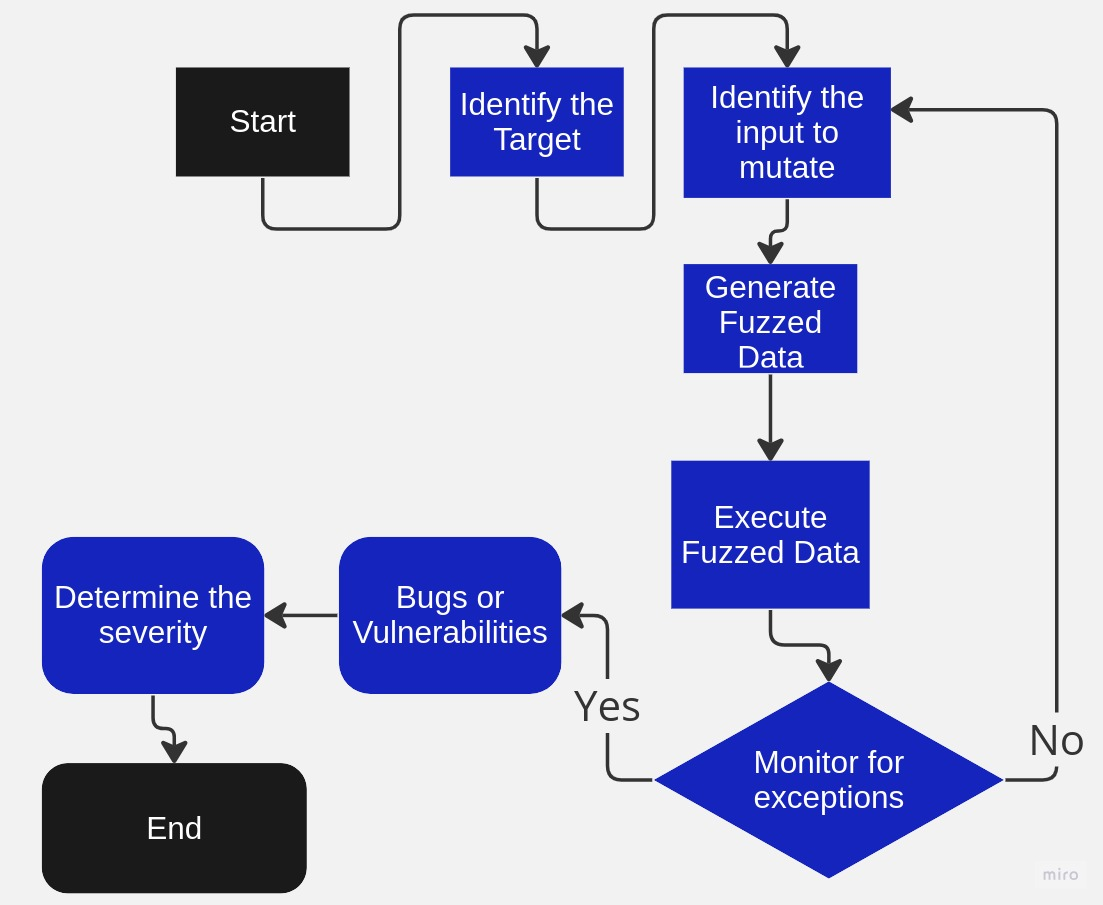
\includegraphics{fuzzy_testing_phases_1}}
        \caption{Fuzzing Stages\cite{segedyfuzz}\cite{9742291}}\label{fig:fuzzy_testing_phases_1}
\end{figure}

Overall, the use of fuzzy testing provides a valuable approach to identifying potential
vulnerabilities in software systems. By generating many test cases with both
valid and malformed data, fuzzing techniques can expose weaknesses in software that may not be
detected through traditional testing methods. Additionally, the analysis of the results of the
fuzzing process enables software developers to identify and address potential security issues
before they can be exploited by malicious actors.

\subsection{History and Evolution of Fuzzy Testing}
The term ``fuzzing'' or ``fuzz testing'',although a relatively recent addition
to the lexicon of automation techniques, was first introduced by Barton Miller
in 1988 as part of a class project\cite{takanen2009fuzzing}. Initially,
fuzzing was perceived as an ad-hoc or random testing method used within
mission-critical applications\cite{WhatisaM24:online}. Over time, however, it
has developed into a specialized technique for the automated generation and
testing of extensive sets of input values for software systems\cite{bohme2020fuzzing}.

The advent of the first open-source fuzz testing framework in 2007\cite{takanen2009fuzzing}
marked a significant evolution in formalizing fuzzing as an approach to software testing.
This led to the creation of a myriad of additional frameworks and tools, expanding the
application of fuzz testing across a diverse set of software systems.

Since its inception, fuzzing has considerably broadened its capacities.
Initially, it was utilized mainly to uncover memory corruption bugs. However,
as discussed by \Citeauthor{bohme2020fuzzing}, its functionality has
evolved over time to include the identification of a diverse range of
software vulnerabilities\cite{bohme2020fuzzing}. \Citeauthor{takanen2009fuzzing} and \Citeauthor{vidas2019fuzzy}
explain that the flexibility and customization capabilities of modern fuzzing
frameworks enable their application across various software layers,
aking fuzzing a potent tool for identifying potential weak spots in
software systems\cite{takanen2009fuzzing}.

Fuzzing techniques have evolved beyond mere bug detection, becoming an essential
tool for vulnerability discovery and, potentially, exploitation.
As indicated by \citeauthor{beaman2022fuzzing}, fuzzing can be
systematically applied to uncover software vulnerabilities, which
may subsequently become exploitable avenues for security
attacks\cite{beaman2022fuzzing}. The subsequent section, referenced as
Section-\ref{par:success_of_fuzzing}, describes the accomplishments and
vulnerabilities revealed by fuzzing techniques over time.

\subsection{Successes Of Fuzzing}
Fuzzy testing has been extremely effective technique since its inception in the
late 1980s in discovering long-standing bugs, vulnerabilities and improving the
quality and security of software. Over the years, wide range of applications
shown in Section-\ref{par:target_categories}, have been successfully fuzzed
and critical security vulnerabilities have been found that could have been
exploited by malicious actors.\label{par:success_of_fuzzing}

The table:\ref{tab:vulnerabilities_examples} showcases examples of vulnerabilities discovered by
fuzzing tools and affected components.

\begin{table}[h!]
\centering
\begin{tabularx}{\textwidth}{@{}>{\raggedright\arraybackslash}p{2cm}>{\raggedright\arraybackslash}p{3cm}X@{}}
\toprule
\textbf{Fuzzing Tool} & \textbf{CVE ID} & \textbf{Description and Affected Component} \\
\midrule
AFL & CVE-2014-0160 & Heartbleed vulnerability in OpenSSL, affecting the TLS heartbeat extension\cite{durumeric2014matter} \\
\addlinespace
AFL & CVE-2014-6271 & Shellshock vulnerability in the Bash shell, allowing remote code execution\cite{shetty2018shellshock} \\
\addlinespace
libFuzzer & CVE-2016-1839  & Heap buffer overflow in ImageIO, affecting image decoding in macOS and iOS \\
\addlinespace
syzkaller & CVE-2017-2636  & Double fetch vulnerability in the Linux kernel, allowing privilege escalation\cite{wang2017double} \\
\addlinespace
go-fuzz & CVE-2016-3959  & Denial of service vulnerability in Go's standard library, affecting the HTTP/2 implementation \\
\addlinespace
Honggfuzz & CVE-2017-15650  & Heap buffer overflow in Poppler, affecting PDF rendering\cite{haller2013dowsing} \\
\bottomrule
\end{tabularx}
\caption{Examples of Vulnerabilities Discovered by Fuzzing Tools}
\label{tab:vulnerabilities_examples}
\end{table}

%\clearpage
The table:\ref{tab:bugs_found_overview} provides a broader overview of the number of bugs found by
different fuzzing tools in various projects.

\begin{table}[h!]
\centering
\begin{tabularx}{\textwidth}{@{}>{\raggedright\arraybackslash}p{1cm}>{\raggedright\arraybackslash}p{2cm}>{\raggedright\arraybackslash}p{3cm}X@{}}
\toprule
\textbf{Year} & \textbf{Organization/Researchers} & \textbf{Fuzzing Tool/Project} & \textbf{Achievements} \\
\midrule
1999 & OUSPG & PROTOS & Found security vulnerabilities in Voice over IP (VoIP) implementations\cite{roning1999protos} \\
\addlinespace
2007 & Microsoft & SAGE & Found critical vulnerabilities in Windows and Office products and had a remarkable impact at Microsoft\cite{godefroid2012sage} \\
\addlinespace
2010 & Adobe & NA & Vulnerabilities uncovered by fuzzing in Adobe Flash, Reader, and Acrobat\cite{AdobeFla64:online} \\
\addlinespace
2016 & ForAllSecure & Mayhem & Competed in DARPA's Cyber Grand Challenge, identified, patched vulnerabilities in real-time\cite{“Mayhem”62:online} \\
\addlinespace
2019 & Microsoft & Project OneFuzz & Used for fuzzing Azure Cloud\cite{GitHubmi60:online} \\
\addlinespace
2023 & Cross platform & AFL & More than 2000 bugs found in open source projects, including OpenSSL, PHP, Python, and others\cite{american20:online} \\
\addlinespace
2023 & Cross-platform & libFuzzer & More than 1000 bugs found in Chromium, OpenSSL, LibreOffice, and other projects\cite{libFuzze17:online} \\
\addlinespace
2023 & Linux kernel developers & syzkaller & More than 800 bugs found in the Linux kernel\cite{syzkalle20:online} \\
\addlinespace
2023 & Go community & go-fuzz & 200+ bugs found in Go programming language and related projects\cite{GitHubdv6:online} \\
\addlinespace
2023 & Cross-platform & Honggfuzz & Bugs found in various projects, including Google's Android and Chrome, and others\cite{GitHubgo17:online} \\
\addlinespace
2023 & Facebook & Facebook's Sapienz & Automated testing of Android apps, leading to crash fixes and improvements\cite{SapienzI13:online} \\
\addlinespace
2023 & Google & ClusterFuzz & More than 25000 bugs found in Google and Chrome\cite{ClusterF78:online} \\
\addlinespace
2023 & Google & OSS-Fuzz & 36,000+ bugs in over 550 open source projects\cite{ClusterF78:online} \\
\bottomrule
\end{tabularx}
\caption{Overview of Bugs Found by Fuzzing Tools in Various Projects}
\label{tab:bugs_found_overview}
\end{table}

%\clearpage


The table:\ref{tab:embedded_fuzzing_success} includes fuzzing success in embedded systems and IoT devices
specifying whether the fuzzing tools are open-source or closed-source:

\begin{table}[h!]
\centering
\begin{tabularx}{\textwidth}{@{}>{\raggedright\arraybackslash}p{0.5cm}>{\raggedright\arraybackslash}p{1.5cm}>{\raggedright\arraybackslash}p{3.8cm}X>{\raggedright\arraybackslash}p{1.2cm}@{}}
\toprule
\textbf{No.} & \textbf{Fuzzing Tool} & \textbf{Target Systems} & \textbf{Achievements} & \textbf{Source} \\
\midrule
1 & AFLNet & FTP, HTTP, and SMTP implementations in IoT devices & Uncovered vulnerabilities and improved security in IoT devices\cite{lin2020aflnet} & Open-source \\
\addlinespace
2 & IoTcube & IoT devices including smart home appliances, medical devices, and industrial IoT devices & Identified and addressed security issues in IoT devices\cite{kim2019iotcube} & Closed-source \\
\addlinespace
3 & FirmFuzz & Firmware in IoT devices including IP cameras and routers & Discovered 7 previously undisclosed vulnerabilities across 6 different devices\cite{srivastava2019firmfuzz} & Open-source \\
\addlinespace
4 & FUZZY & Zigbee implementations in IoT devices & Identified new security vulnerabilities in Zigbee, a widely used wireless communication protocol for IoT devices\cite{vidas2019fuzzy} & Closed-source \\
\addlinespace
5 & Atheris & Python programs, including embedded systems using MicroPython & Detected various types of vulnerabilities, such as buffer overflows and memory leaks, in Python-based embedded systems\cite{atheris2020} & Open-source \\
\bottomrule
\end{tabularx}
\caption{Fuzzing Success in Embedded Projects}
\label{tab:embedded_fuzzing_success}
\end{table}

%\clearpage

\subsection{Why, How and What to Fuzz}

Fuzzing provides significant insights into the security, robustness,
and resilience of software systems, especially those that interact with inputs
from untrusted sources. While it does not make any guarantees about the
reliability of inputs or transforms an untrusted source into a trusted one,
it helps identify problematic inputs that could cause the software system to
crash or behave
unexpectedly\cite{bohme2020fuzzing}\cite{beaman2022fuzzing}\cite{vidas2019fuzzy}\cite{WhatisFu63:online}.

It's crucial to emphasize that fuzz testing doesn't necessarily affirm the
correctness of complex software programs. Instead, it contributes to the
understanding of the system's behavior under diverse and unexpected input
conditions. Particularly for software playing a critical role in larger
systems or applications, fuzz testing can highlight unforeseen
issues\cite{fuzzinga40:online}\cite{demott2006evolving}\cite{WhatisFu63:online}.

Moreover, fuzz testing aids in assessing the software system's stability under
stress. By exposing the software to high volumes of varied inputs, this
technique can identify potential performance or stability issues, arising
from heavy usage or stress conditions\cite{demott2006evolving}.

However, it's important to understand that fuzzing is not a panacea for
all software flaws. It's a specialized tool aimed at discovering errors
and vulnerabilities that might not directly relate to the software's
requirements or intended functionalities. While it's effective at uncovering
specific issues like memory leaks\cite{shahriar2014testing},
address corruptions\cite{muench2018you}, and buffer overflows\cite{godefroid2020fuzzing},
it should complement other types of testing such as functional, unit,
integration, and system testing, rather than replace
them\cite{pietikainen2016steps}\cite{UnitTest25:online}\cite{WhatisFu63:online}.

To leverage fuzzing effectively, careful planning is essential to identify
specific targets for testing. Notably, identifying and defining entry points
for fuzzing in large and complex applications can be challenging but essential.
These entry points, including file inputs, network inputs, and command
line inputs, help fuzz testers concentrate their efforts on the areas
most susceptible to potential issues\cite{oehlert2005violating}.
Thus, the meticulous selection of
fuzz testing targets is instrumental to the test's success, underpinning
thorough testing of the most vulnerable software components.

Below given examples applications targets where fuzzing has been successful\cite{fuzzingw44:online}.\label{par:target_categories}

\begin{itemize}
        \item Databases: SQLite\cite{fu2022griffin}
        \item Text editors: VIM\cite{FuzzingV8:online}, OpenOffice\cite{Presenta60:online}
        \item Media codecs: audio, video, raster and vector images\cite{thiel2008exposing}\cite{rhodenfuzzing}
        \item Linux OS kernels, drivers\cite{schumilo2017kafl}\cite{corina2017difuze}
        \item Parsers: xml, pdf\cite{wang2017skyfire}
        \item Crypto libraries: OpenSSL\cite{opensslR89:online}, LibreSSL\cite{GitHubli9:online}
        \item Browsers: Chrome\cite{Fuzztest23:online}, Firefox\cite{Fuzzing—21:online}
        \item Network protocols\cite{GitHubnc82:online}, scanners\cite{SnapFuzz27:online}
\end{itemize}


\section{Fuzzing Process, Components, and Various Approaches}\label{sec:fuzzing_methods}
Fuzzing, a dynamic software testing technique, plays a crucial role in enhancing
software reliability and security by detecting concealed bugs and
vulnerabilities. Its importance has grown in tandem with the increasing
complexity and pervasiveness of software systems, making it a prominent
field of academic and practical interest. This section provides an exhaustive
exploration of the fuzzing process, including its various stages, the evolution
of its techniques, and the methodologies employed.

\subsection{Test Case Generation: From Basic to Advanced Techniques}
The process of fuzzing commences with the generation of numerous inputs
designed to provoke the program's failure. These inputs can take various forms,
including different file formats, binary executables, or network commands
\cite{mcnally2012fuzzing}\cite{bohme2020fuzzing}\cite{manes2019art}.
Generating broken inputs that can trigger a program to fail presents a
significant challenge, which is tackled through mutation-based\cite{miller2007analysis}\cite{lyu2022ems} and
generation-based generators\cite{pang2023generation}.

Mutation-based fuzzing represents an evolution from primitive fuzzing techniques
that relied heavily on generating inputs through random bytes.
In contrast, mutation-based fuzzing utilizes existing input data,
also known as a test corpus, and tweaks it to create new test data\cite{miller2007analysis}.
These mutation algorithms can vary significantly, with some employing
stochastic modeling to concentrate mutations on specific parts of the input\cite{lyu2022ems}\cite{miller2007analysis}.


Generation-based generators, on the other hand, fabricate entirely new inputs
for fuzzers, making them an essential tool in the fuzzing
process\cite{li2018fuzzing}\cite{miller2007analysis}\cite{wang2017skyfire}.

\subsection{Execution and Monitoring: Coverage-Guided Fuzzing and Sanitizers}
Upon generating the inputs, the test cases are fed to the program, and the
fuzzing process persists until the occurrence of a program crash or hang. This
stage involves monitoring crashes and exceptions using tools like
sanitizers\cite{GitHubgo55:online}\cite{osterlund2020parmesan}, which can detect specific system signals,
crashes, and other violations.

\textbf{Sanitizers}
\newline
Sanitizers are integral components in the process of fuzzing. They assist in
locating bugs which do not necessarily lead to a crash. However, they are
resource-intensive, increasing both CPU\cite{WhatisaC78:online} and
RAM\cite{WhatisRA11:online} usage. Therefore, usage of
sanitizers should be carefully managed to avoid excessive resource utilization.

\begin{itemize}

\item \textit{Address Sanitizers (ASAN)\cite{AddressS43:online}:} These tools
are crucial in identifying vulnerabilities related to memory corruption such
as use-after-free, NULL pointer dereferences, and buffer overflows\cite{haller2013dowsing}.

\item \textit{Memory Sanitizers (MSAN)\cite{MemorySa64:online}:} They serve to
detect unauthorized read accesses to uninitialized memory, such as when a local
variable is defined and read before being set\cite{stepanov2015memorysanitizer}.

\item \textit{Undefined Behavior Sanitizers (UBSAN)\cite{Undefine50:online}:} These sanitizers help in
identifying instances of undefined behavior as per the C and C++ standards,
such as when the result of an operation exceeds the permissible limit of a data type.
\end{itemize}


Coverage-guided fuzzing\cite{jaaskela2016genetic} is another crucial part of
the execution and monitoring stage. This method involves tracking how much and
which sections of the \acrshort{sut} are covered by the inputs throughout the
fuzzing campaign. Compiler instrumentation, utilized by fuzzers such as
AFL/AFL++\cite{257204} or libFuzzer\cite{libFuzze17:online}, is often
employed to gather this data. External function calls are injected into
specific points during the compilation process to relay data to the fuzzer each
time an edge or block is encountered\cite{libFuzze17:online}\cite{bohme2016coverage}\cite{257204}.

Figure\ref{fig:feedback-based-fuzzing} depicts a simple visual representation of the
feedback based fuzzing.

% \begin{figure}[ht]
% \centering
% \AltText{Feedback Based Fuzzing}{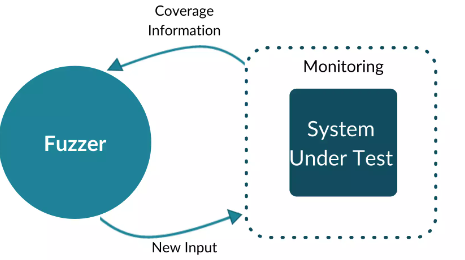
\includegraphics[width=8.5cm, height=5.5cm]{feedback-based-fuzzing}}
% \caption{Feedback Based Fuzzing\cite{TheMagic36:online}\cite{LucianoR49:online}}\label{fig:feedback-based-fuzzing}
% \end{figure}

\begin{figure}[h]
        \centering
        \adjustbox{width=\textwidth}{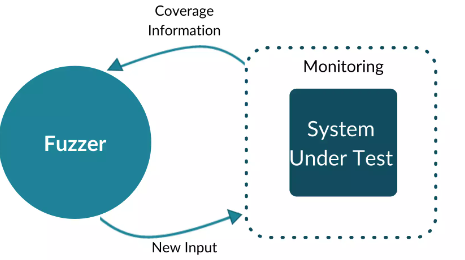
\includegraphics{feedback-based-fuzzing}}
        \caption{Feedback Based Fuzzing\cite{TheMagic36:online}\cite{LucianoR49:online}}\label{fig:feedback-based-fuzzing}
\end{figure}

\subsection{Analysis: Discovering and Filtering Bugs}
The analysis stage concentrates on identifying the root cause of issues
detected during the monitoring phase. This stage involves both the bug
detector\cite{liang2018fuzzing}\cite{bekrar2012taint}, a key component in fuzzers
designed to identify potential bugs,
and the bug filter\cite{peng2018t}\cite{bekrar2012taint}\cite{chen2013taming},
which works to filter out non-security related bugs
from the overall reported bugs. The bug detector collects and analyzes the
stack traces from the crashes and errors that occur as a result of the test
inputs, while the bug filter helps sift through these findings to prioritize
security-related bugs.

\subsection{Visibility in Fuzzing}

The term ``Visibility'' in fuzzing refers to the degree of information about the
\acrshort{sut} exposed to the fuzzer's runtime. There are three primary visibility levels in
fuzzing: Blackbox\cite{godefroid2007random}\cite{manes2019art},
Graybox\cite{canakci2021directfuzz}\cite{li2018fuzzing}, and
Whitebox\cite{godefroid2008automated}\cite{godefroid2007random}\cite{godefroid2008grammar} fuzzing,
each offering different degrees of access to the source code of the \acrshort{sut}.

Through the synthesis of these techniques-mutation-based\cite{lyu2022ems}\cite{miller2007analysis}
test case generation, coverage-guided\cite{jaaskela2016genetic} execution and monitoring, comprehensive bug analysis,
and the consideration of visibility levels-fuzzing becomes a powerful tool
for enhancing the overall software quality and security. By identifying and
addressing the root cause of software bugs and vulnerabilities, developers
can prevent these issues from being exploited by attackers.

The figure-\ref{fig:general_process_fuzzing} offers a visual representation of the
fuzzing process and its dependencies.

% \begin{figure}[ht]
% \centering
% \AltText{General Process Fuzzing}{\includegraphics[width=12.1cm][height=20.1cm]{general_process_fuzzing}}
% \caption{General Process Fuzzing\cite{liang2018fuzzing}.}\label{fig:general_process_fuzzing}
% \end{figure}

% \begin{figure}[ht]
% \centering
% \AltText{General Process Fuzzing}{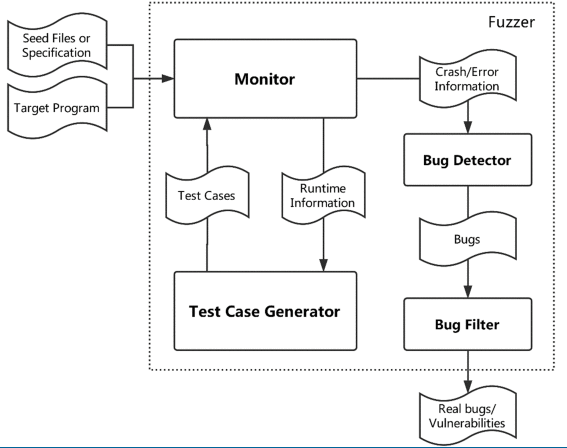
\includegraphics[width=14.5cm, height=20.5cm]{general_process_fuzzing}}
% \caption{General Process Fuzzing\cite{liang2018fuzzing}}\label{fig:general_process_fuzzing}
% \end{figure}

\begin{figure}[h]
        \centering
        \adjustbox{width=\textwidth}{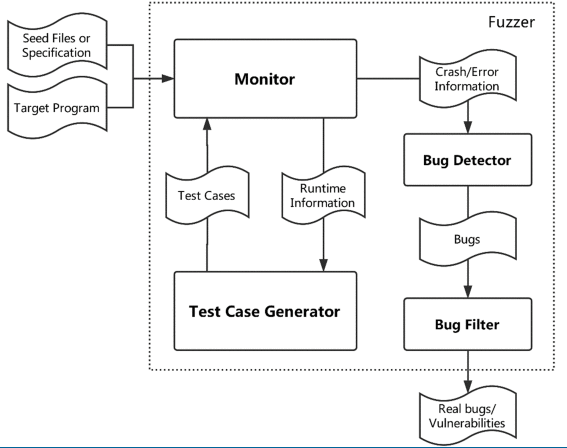
\includegraphics{general_process_fuzzing}}
        \caption{General Process Fuzzing\cite{liang2018fuzzing}}\label{fig:general_process_fuzzing}
\end{figure}

As the target of a fuzzing test, the \acrshort{sut}, typically a binary program,
is meticulously scrutinized by fuzzers. The generated inputs for the fuzzing process,
derived from either mutation-based or generation-based methods, comprise a mixture of valid and
invalid inputs that pass initial validation but may still trigger bugs. The process is dynamic
and continuously evolving, with ongoing research aimed at improving and automating the various
stages, from input generation to bug detection and filtering.
%\clearpage


% \section{Classification of Fuzzing Methods}\label{sec:fuzzing_methods}
% Fuzzing tools and methods are classified into three main categories: gray-box, white-box and
% black-box fuzzing.

% \subsection{White-Box Fuzzing Method}

% White-box fuzzing is a systematic technique for enumerating different interesting paths in a
% program by using program analysis and constraint solvers. It relies on the internal logic
% of the target program and is based on the technique called \textit{symbolic execution}\cite{cadar2013symbolic}.
% This method was proposed to overcome the limitations of black-box fuzzing and was first
% \Citeauthor{godefroid2008automated}. To scan through the target program, white-box fuzzing uses
% a search technique called coverage-maximizing heuristic search
% algorithm\cite{godefroid2008automated}\cite{liang2018fuzzing}.

% Before starting the fuzzing process, white-box fuzzing requires the necessary information
% from the target program to generate the inputs. It collects all the conditional paths of the target
% program by applying \acrlong{smt} formulas. For example, it uses the formula
% \begin{math}i[0] = 42 \land i[0] - i[1] > 7\end{math}, where \textit{i} is the set of inputs
% that traverse the target\cite{bohme2021fuzzing}. The path condition is then calculated and mutated
% and sent to a constraint solver to generate new paths and skip the blocks.
% The main goal of white-box fuzzers is to reach the maximum execution paths and requirements.


% One of the advantages of white-box fuzzing is that it can cover maximum coverage by generating
% better and more interesting test cases. However, numerous execution paths can lead to stability and
% compatibility issues in real-world software\cite{lomeli2022security}\cite{liang2018fuzzing}.
% Some existing white-box fuzzers are SAGE\cite{godefroid2012sage}, KLEE\cite{cadar2008klee},
% BitFuzz\cite{caballero2010input}.\newline

% \subsection{Black-Box Fuzzing Method}
% Black-box testing method involves generating inputs to test the target program without any
% internal knowledge or specifications. The fuzzing process begins by randomly mutating
% the valid inputs or generating new inputs. Examples of mutation data include flipping random bits
% and bytes in a seed file, byte copies, and removal\cite{jaaskela2016genetic}.
% Generational-based approaches utilize grammar and input-specification knowledge\cite{kim2013automatic}.

% The fuzzing process ends after a predefined time has been exhausted. Popular black-box fuzzers
% include Peach\cite{PeachFuz35:online}, Trinity\cite{GitHubke76:online} and
% Funfuzz\cite{GitHubMo73:online}.\newline

% \subsection{Gray-Box Fuzzing Method}
% The combination of black-box and white-box fuzzing utilizes \textit{code instrumentation}
% to provide feedback and obtain code coverage of the target program during runtime\cite{bohme2021fuzzing}.
% This approach employs genetic algorithm mutation strategies to generate new inputs which serve as
% new control locations to cover additional coverage paths. Feedback received from the coverage
% enables the fuzzers to reach more coverage, including tracing the taint data flow, in a method known
% as gray-box \textit{taint-analysis}\cite{bekrar2012taint}.

% To detect bugs and vulnerabilities, assertions are injected by sanitizers into the target program.
% Unlike the white-box method, the gray-box method utilizes runtime information to generate test cases.
% Some well-known gray-box fuzzers include AFL++\cite{257204}: a fork
% of \gls{afl}\cite{GitHubgo92:online}, LibFuzzer\cite{libFuzze17:online} and Honggfuzz\cite{GitHubgo89:online}.\newline

% \subsection{Choose a Fuzzing Method}
% In software testing, a `bug' refers to a defect in the software logic that causes unexpected or
% incorrect output. The primary objective of fuzz testing is to identify and eliminate such bugs
% in a system. In order to achieve this objective, selecting an appropriate fuzzing target is of
% utmost importance. While black-box fuzzers are simple and lightweight, they may not be capable
% of achieving high levels of code coverage and are more effective in uncovering `shallow`
% bugs. On the other hand, white-box and gray-box fuzzers are adept at detecting  `hidden' bugs
% that are difficult to identify. Although the implementation of these fuzzers is more complex
% and time-consuming, they offer comprehensive and in-depth testing capabilities.

% When considering fuzz testing methods, two important factors to consider are precision and efficiency,
% as well as the quality of the results. A `dumb' fuzzer simply mutates a valid input by
% randomly changing some bytes, while a `smart' fuzzer generates inputs from scratch.
% The black-box fuzzing approach is known for its precision and efficiency, while the white/gray
% box methods tend to produce higher quality results. Careful consideration of these factors is
% essential when selecting an appropriate fuzz testing method for a given software system.

% The two factors are:
% \begin{enumerate}
%         \item Time and Budget
%         \item Input format of the target program e.g, network protocol, compiler
% \end{enumerate}

% \section{Implementing the Art of Fuzzing}
% As per the section \hyperref[sec:fuzzing_methods]{Classification of Fuzzing Methods} below questions\cite{liang2018fuzzing}
% should be considered when building and implementing fuzzing with fuzzers.

% \begin{itemize}
%         \item How to do seed selection and generation.
%         \item What makes a good \gls{fuzz_target} and how to validate the inputs.
%         \item What to consider with the test cases which indicates crashes.
%         \item How to make good use of information during the runtime.
%         \item How can we achieve scalability improvements.\newline
% \end{itemize}

% \subsection{Generation and Selection of Seed}

% In the field of fuzz testing, the term \textit{seed corpus} denotes an assortment
% of representative input files that a target program is designed to process.
% The composition of the seed corpus can profoundly influence the efficacy and efficiency
% of the fuzzing process, emphasizing the importance of its selection for
% maximizing test coverage\cite{herrera2021seed}.

% Striving for high coverage implies the goal to activate and evaluate as
% many code paths as possible within the target program during the fuzzing process.
% While 100\% coverage represents a theoretical ideal, practically achieving this
% level of thoroughness is rare due to the intricate and expansive nature of
% modern software. Nevertheless, aiming for high coverage substantially enhances
% the probability of revealing concealed bugs and vulnerabilities, thus providing
% a comprehensive evaluation of the system's reliability and security\cite{godefroid2012sage}.

% The size of the seed corpus necessitates a careful balancing act between file
% size and coverage. While larger seed files may offer greater potential for
% coverage, they consume more computational resources and processing time. Smaller
% seed files, processed more rapidly, might not deliver the same level of coverage.
% Therefore, if a smaller seed file yields similar coverage to a larger one, its
% usage is preferable for improved testing
% efficiency\cite{liang2018fuzzing}\cite{jurczyk2016effective}. Nonetheless,
% in scenarios with ample storage capacity—either physical or cloud—larger seed
% files can be utilized, often compressed to conserve space without compromising
% the comprehensive representation of potential program inputs\cite{liang2018fuzzing}.

% The selection of the seed corpus typically precedes the fuzzing process,
% particularly crucial when employing a mutation-based fuzzer. This type of fuzzer
% requires an initial set of inputs or \textit{seed corpus} to commence testing.
% The quality of these initial seeds significantly influences the fuzzer's capacity
% to explore the program's state space and detect bugs\cite{miller2007analysis}.

% Moreover, a method for enhancing code coverage, as
% proposed by\Citeauthor{kim2011efficient}\cite{kim2011efficient},
% involves an in-depth analysis of binary file fields during fuzzing.
% This strategy entails tracking and evaluating stack frames, assembly codes,
% and registers to unearth potential new inputs that could augment coverage.

% In summary, the careful selection of a suitable seed corpus is a vital
% component of effective fuzz testing. The goal is to optimize coverage while
% considering the constraints of file size and storage capacity. Particularly in
% mutation-based fuzzing, a well-chosen seed corpus can lead to a more efficient and
% comprehensive exploration of the target program.


% \subsection{A Good Fuzz Target and Validation of Inputs}
% In the context of fuzz testing, the term `fuzz target' refers to the item being tested.
% This item can take many forms, such as a command line tool or a hardware device, and is
% characterized by its ability to accept inputs and provide results. The effectiveness of
% the fuzz testing process depends on the quality of the fuzz target and its ability to
% accurately represent the behavior of the real-world system or application being tested\cite{238602}.

% \subsubsection{A Good Fuzz Target}
% Below given is an example of a fuzz target written in C with \textit{LLVM libFuzzer}\cite{libFuzze17:online},
% \begin{minted}[linenos,frame=lines,baselinestretch=1.2,breaklines]{c}

% extern "C" int LLVMFuzzerTestOneInput (const uint8_t *Data, size_t Size) {
%         DoSomethingInterestingWithMyAPI(Data, Size);
%         return 0;  // Values other than 0 and -1 are reserved for future use.
% }

% \end{minted}

% The function \textit{LLVMFuzzerTestOneInput} of the fuzzer \textit{libFuzzer} takes two arguments,
% the address of the data to store and size. The API of the fuzz target is called in the next steps of
% fuzzing.

% It is crucial to keep the following aspects in mind when creating a fuzz target\cite{libFuzze17:online}\cite{257204}:

% \begin{itemize}
% \item The \gls{fuzzing_engine} needs to be designed so that it can execute the fuzz target multiple times within the same process, enhancing efficiency.
% \item The fuzz target should be able to handle a wide range of inputs, from valid to malformed and even empty inputs, increasing its robustness.
% \item An abrupt halt or unexpected exit from the fuzz target typically indicates a bug within the system. Thus, these instances warrant close monitoring.
% \item To expedite testing, the fuzz target's execution speed should be optimized. Furthermore, it should be designed to consume minimal memory, avoiding the risk of out-of-memory errors.
% \item If the fuzz target relies on a global state, it should be designed to avoid modifying it. For instance, the use of \textit{malloc()} could inadvertently modify the global state.
% \item To foster a culture of regular testing, the fuzz target should be integrated into a \textit{continuous integration} system.
% \item Consistent results are key in fuzzing. Consequently, the fuzz target should be deterministic, meaning that it should not rely on random factors that could lead to inconsistent outcomes.
% \item The fuzz target should be designed for speed as the fuzzing process requires multiple iterations. Therefore, its performance can significantly impact the testing speed.
% \item The memory consumption of the fuzz target should be kept minimal to avoid running into out-of-memory errors which could disrupt the testing process.
% \item It is essential to ensure the fuzz target is designed in a way that avoids conditions that could lead to timeouts and out-of-memory errors, thus ensuring smooth and uninterrupted testing.
% \end{itemize}

% \subsubsection{Input Validations}
% Fuzzing offers the main advantage of generating test cases quickly. However, when the fuzz target
% being tested has input validations, the generated test cases may not be useful. Hence, it is
% crucial to exercise caution when creating test cases in such scenarios.

% \textbf{Integrity Validation:}
% Integrity validation is a crucial aspect of maintaining data integrity in various inputs
% such as file formats and network protocols. To ensure the integrity of the data,
% checksum mechanisms are used, which provide validation at both the sending and receiving ends.
% In this regard, a fuzzer named \textit{TaintScope}, developed by \citeauthor{wang2010taintscope},
% is used to mutate the hot bytes in the input, which helps in generating new test cases. However, to pass the
% integrity validation, the checksum is reverted to its original state. This approach enables
% the detection of vulnerabilities that might arise in the process of transmitting data,
% which could compromise the integrity of the system\cite{wang2010taintscope}.

% \textbf{Format Validation:}
% Fuzz targets such as Android devices, compilers, and interpreters have format requirements that
% must be met by inputs in order to be accepted for testing. However, in cases where inputs
% do not conform to these formats, they are rejected by the system. To avoid format-based validation,
% a \textit{Grammar}-based solution can be employed. For instance, \Citeauthor{cao2015towards},
% developed a scanner for fuzz targets on Android devices, which is capable of evading the
% initial format validation and allowing the fuzz testing process to continue without
% interruption\cite{cao2015towards}.

% \textbf{Environment Validation:}
% Environment validation is a crucial aspect of testing, which checks the validity of configurations,
% runtime status, and other environmental factors. Fuzzing tools, such as FuzzDroid\cite{rasthofer2017making},
% utilize a combination of static and dynamic analysis to generate an Android runtime environment.
% The tool employs a search-based algorithm to identify potential vulnerabilities, which helps in
% enhancing the overall security of the system. Through this approach, FuzzDroid can effectively
% identify and address issues related to syntactic and semantic validity, ultimately improving the
% reliability and performance of the system.


% \textbf{Input Coverage:}
% Achieving high input coverage is critical to uncovering vulnerabilities in a target system.
% Various techniques have been proposed to improve the input coverage of a fuzzer.
% One such tool is the \textit{semi-valid coverage (SVCov)} tool, proposed by  \Citeauthor{tsankov2013semi},
% SVCov helps increase the existing input coverage by generating inputs that are close to
% valid inputs but still contain errors or faults that can trigger bugs in the system under test\cite{tsankov2013semi}.

% Another technique to enhance input coverage is through the use of specialized fuzzers such as \textit{Artfuzz},
% which was proposed by \Citeauthor{chen2016dynamically}. Artfuzz is designed to find non-crash buffer overflow
% vulnerabilities by identifying inputs that can trigger buffer overflows but do not cause the system to crash.
% By uncovering such vulnerabilities, Artfuzz helps improve the security of the target system\cite{chen2016dynamically}.

% \subsubsection{Isolating Crashes and Test Cases}
% Fuzzing often causes crashes in the target systems. These crashes can be huge in numbers and often
% takes a large amount of time for analyzing. Due to time and budget often the most priority bugs get
% fixed by the developers. Therefore, it is really important for the testers to isolate or filter
% the test inducing crashes and take the most useful test cases into account.

% \Citeauthor{chen2013taming} introduced a ranking based to isolate the crashes and test cases\cite{chen2013taming}.
% In this method, the test cases which can cause bugs, and they are different in nature are ranked accordingly.
% There are other methods for isolating the crashes such as clustering methods, differentiating the crashes based
% on their uniqueness and debug information. The stack traces play an important role in determining the uniqueness
% of the test cases and therefore need to recorded while doing the fuzzing. Another simpler way to determine the
% uniqueness is to trace the execution path. Fuzzers like AFL\cite{GitHubgo92:online} determines a crash is unique
% when it does not find the execution path. The uniqueness helps in isolating the crashes, the outputs and saves
% time when analyzing them. Trimming of the test cases is another method of isolating the crashes and test cases.
% A large size test case can take more time to execute and then more time for analysis. In mutation based fuzzers,
% in which the test cases are developed and mutated during the run time usually fall into this category. Hence, trimming
% of the test cases is needed from time to time while fuzzing and which can improve the overall efficiency. Trimming
% is usually done by removing the identical data-blocks which can not influenced the execution path anymore
% by comparing them with the original one.

% \subsubsection{Runtime Information During Fuzzing}
% To get code coverage and data flow which are runtime information,  symbolic execution and dynamic
% analysis techniques are used. Although these techniques help in finding the `hidden' bugs, these smart
% fuzzing techniques are low in efficiency.


% Path Explosion is one of the biggest problem in symbolic execution during fuzzing run time. A conditional branch
% in any target program can have a numerous execution paths and this can lead to Path Explosion.
% \Citeauthor{godefroid2007compositional} proposed to have \textit{function summaries} in low level
% functions. This can lead to less number of execution paths as the higher level functions can
% reuse them\cite{godefroid2007compositional}. Heuristic search algorithms such as random path selection
% and automatic partial loop summarization help to find the most relevant paths\cite{liang2018fuzzing}.

% Complex programs can cause imprecision symbolic execution. Methods such as CUTE\cite{sen2005cute} helps
% in making the symbolic execution more cost effective.

% During the runtime, \textit{Undertainting} is another problem where without any direct assignment The
% variable is transferred. \Citeauthor{kang2011dta++} has proposed that to Undertainting, it is essential to
% neglect the input data flow if the input is tainted\cite{kang2011dta++}.


% \subsubsection{Isolating Crashes and Test Cases}

% Fuzzing frequently leads to numerous system crashes, which can be cumbersome and
% time-consuming to analyze. As a result of time and budget constraints,
% prioritization becomes crucial; hence, testers must effectively isolate
% and filter crash-inducing test cases. \Citeauthor{chen2013taming} proposed a
% ranking-based method to categorize these cases based on their bug-inducing
% capabilities and their distinctiveness\cite{chen2013taming}.

% Isolation of crashes can also be achieved through clustering methods,
% differentiating crashes based on uniqueness and debug information. Stack
% traces and execution path tracing are essential in determining the uniqueness
% of the test cases. For instance, AFL uses the absence of a pre-existing execution
% path to define the uniqueness of a crash\cite{GitHubgo92:online}.

% Trimming is another approach employed to optimize the fuzzing process. Large
% test cases, often generated in mutation-based fuzzers, could potentially slow
% down execution and analysis. To counter this, identical data-blocks that no
% longer influence the execution path are removed periodically, thereby enhancing
% overall efficiency.

% \subsubsection{Runtime Information During Fuzzing}

% Smart fuzzing techniques like symbolic execution and dynamic analysis are used
% to gather runtime information such as code coverage and data flow, although
% their efficiency can be limited. One significant challenge is path explosion,
% a phenomenon caused by the numerous execution paths stemming from a single
% conditional branch in the target program.

% \Citeauthor{godefroid2007compositional} suggested the use of `function summaries'
% for lower-level functions to reduce the number of execution paths, allowing
% higher-level functions to reuse them\cite{godefroid2007compositional}.
% Additionally, heuristic search algorithms like random path selection and
% automatic partial loop summarization help to identify the most relevant paths\cite{liang2018fuzzing}.


\section{Implementing the Art of Fuzzing}
Based on the classification of fuzzing methods delineated in
section \hyperref[sec:fuzzing_methods]{Classification of Fuzzing Methods},
several questions arise when constructing and implementing fuzzing with
fuzzers\cite{liang2018fuzzing}:

\begin{itemize}
\item How to select and generate seeds?
\item What characteristics define a good \gls{fuzz_target}, and how can one validate the inputs?
\item What considerations should be taken into account when dealing with test cases causing crashes?
\item How to effectively utilize information during runtime?
\item How to achieve scalability improvements?
\end{itemize}
The responses to these queries determine the effectiveness of fuzzing in
revealing hidden vulnerabilities, thereby enhancing the security and reliability of the target system.

\subsection{Generation and Selection of Seed}

Seed corpus in fuzz testing refers to a collection of representative input
files that the target program is designed to process. The seed corpus selection
can significantly influence the efficacy and efficiency of the fuzzing process,
emphasizing its importance for maximizing test coverage\cite{herrera2021seed}.

In an ideal scenario, a fuzzer aims for 100\% coverage, seeking to activate and
examine as many code paths as possible within the target program. However, this
is rarely achieved due to the complex and large-scale nature of contemporary
software. Nonetheless, striving for high coverage significantly improves the
chances of uncovering hidden bugs and vulnerabilities, enhancing the evaluation
of system reliability and security\cite{godefroid2012sage}.

The size of the seed corpus must be chosen with careful consideration of
its potential effect on coverage and computational resources. Larger seed files
may provide more coverage but consume more resources and time. If smaller seed
files can provide similar coverage to larger ones, they are typically preferred
for efficient testing\cite{liang2018fuzzing}\cite{jurczyk2016effective}.

The initial seed corpus is particularly crucial when using a mutation-based
fuzzer, which requires an initial set of inputs or seeds. The quality of these
seeds substantially influences the fuzzer's capacity to explore the program's
state space and detect bugs\cite{miller2007analysis}. An efficient way of
enhancing code coverage, proposed by \Citeauthor{kim2011efficient}, involves a
detailed analysis of binary file fields during fuzzing. This approach includes
tracking and evaluating stack frames, assembly codes, and registers to unearth
potential new inputs that could augment coverage\cite{kim2011efficient}.

\subsection{A Good Fuzz Target and Validation of Inputs}
In the context of fuzz testing, the `fuzz target' is the item being tested.
This can be anything from a command line tool to a hardware device. The quality
of the fuzz target is crucial as it should accurately represent the behavior of
the real-world system or application being tested\cite{238602}.

\subsubsection{A Good Fuzz Target}
Here is an example of a fuzz target written in C with LLVM libFuzzer\cite{libFuzze17:online}:

\begin{minted}[linenos,frame=lines,baselinestretch=1.2,breaklines]{c}

extern "C" int LLVMFuzzerTestOneInput (const uint8_t *Data, size_t Size) {
DoSomethingInterestingWithMyAPI(Data, Size);
return 0; // Values other than 0 and -1 are reserved for future use.
}

\end{minted}

In this case, the function \textit{LLVMFuzzerTestOneInput} takes two arguments,
the address of the data to store and its size. The API of the fuzz target is
called in subsequent steps of fuzzing. When creating a fuzz target, the
following aspects should be taken into account\cite{libFuzze17:online}\cite{257204}:

\begin{itemize}
\item The \gls{fuzzing_engine} should be designed to execute the fuzz target
multiple times within the same process to enhance efficiency.
\item The fuzz target should handle a wide range of inputs, from valid to
malformed and even empty, to increase robustness.
\item Any abrupt halt or unexpected exit from the fuzz target usually
signifies a bug within the system and warrants closer examination.
\item For faster testing, the fuzz target's execution speed should be
optimized. Moreover, it should consume minimal memory to avoid out-of-memory errors.
\item If the fuzz target relies on a global state, it should be
designed to avoid altering it.
\item Regular testing should be encouraged by integrating the fuzz
target into a continuous integration system.
\item The fuzz target should be deterministic to ensure consistent results.
\item It is crucial to optimize the performance of the fuzz target as the
fuzzing process requires multiple iterations.
\end{itemize}

\subsubsection{Isolating Crashes and Test Cases}

Fuzzing often results in many system crashes, which can be challenging and
time-consuming to analyze. Therefore, due to time and budget constraints, it's
important to isolate and filter crash-inducing test cases effectively. A
ranking-based method to categorize these cases based on their bug-inducing
capabilities and distinctiveness was proposed by \Citeauthor{chen2013taming}\cite{chen2013taming}.

Crashes can also be isolated through clustering methods, differentiating
crashes based on uniqueness and debug information. For example, AFL uses the absence
of a pre-existing execution path to define the uniqueness of a crash\cite{GitHubgo92:online}.

\subsubsection{Runtime Information During Fuzzing}

Advanced fuzzing techniques, such as symbolic execution and dynamic analysis,
are used to gather runtime information, such as code coverage and data flow.
However, their efficiency can be limited due to challenges like path explosion,
a phenomenon caused by the multiple execution paths that stem from a single
conditional branch in the target program.

\Citeauthor{godefroid2007compositional} suggested using `function summaries'
for lower-level functions to reduce the number of execution paths. This allows
higher-level functions to reuse them\cite{godefroid2007compositional}. Additionally,
heuristic search algorithms like random path selection and automatic partial
loop summarization help identify the most relevant paths\cite{liang2018fuzzing}.

In summary, effective fuzzing implementation requires careful consideration of
various factors. The seed selection and generation, quality of the fuzz target,
test case management, use of runtime information, and scalability all play
significant roles in the process. Employing advanced techniques and maintaining
a clear focus on these aspects can optimize the fuzzing process and enhance its
ability to uncover hidden bugs and vulnerabilities in the target system.
\clearpage